\chapter{Command}
\section{Intento}

Incapsula una richiesta come oggetto, consentendo in tal modo di parametrizzare i client con richieste diverse, richieste di coda o di registro e operazioni non supportabili.

(nel progetto da usare quando si utilizzano delle query)


%---
\section{Prestruttura}

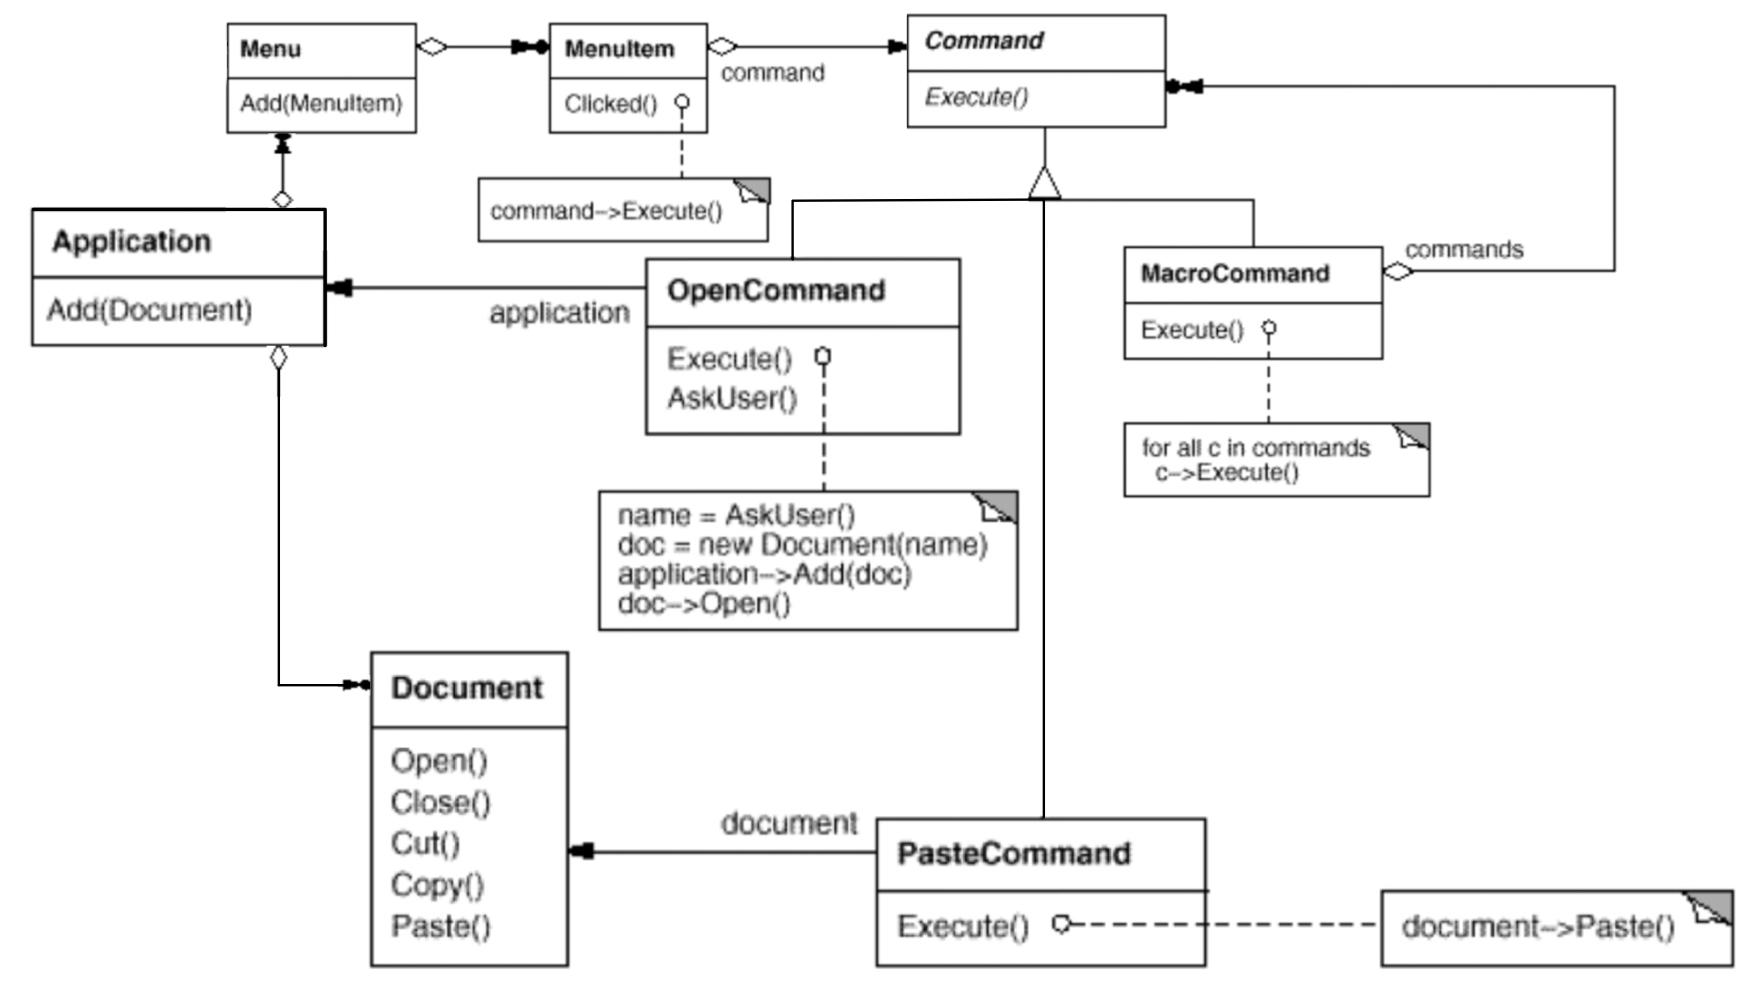
\includegraphics[width=\textwidth]{/Users/matt/Documents/LaTex/Design Pattern LaTex/Command/Prestructure1}


%---
\section{Struttura}

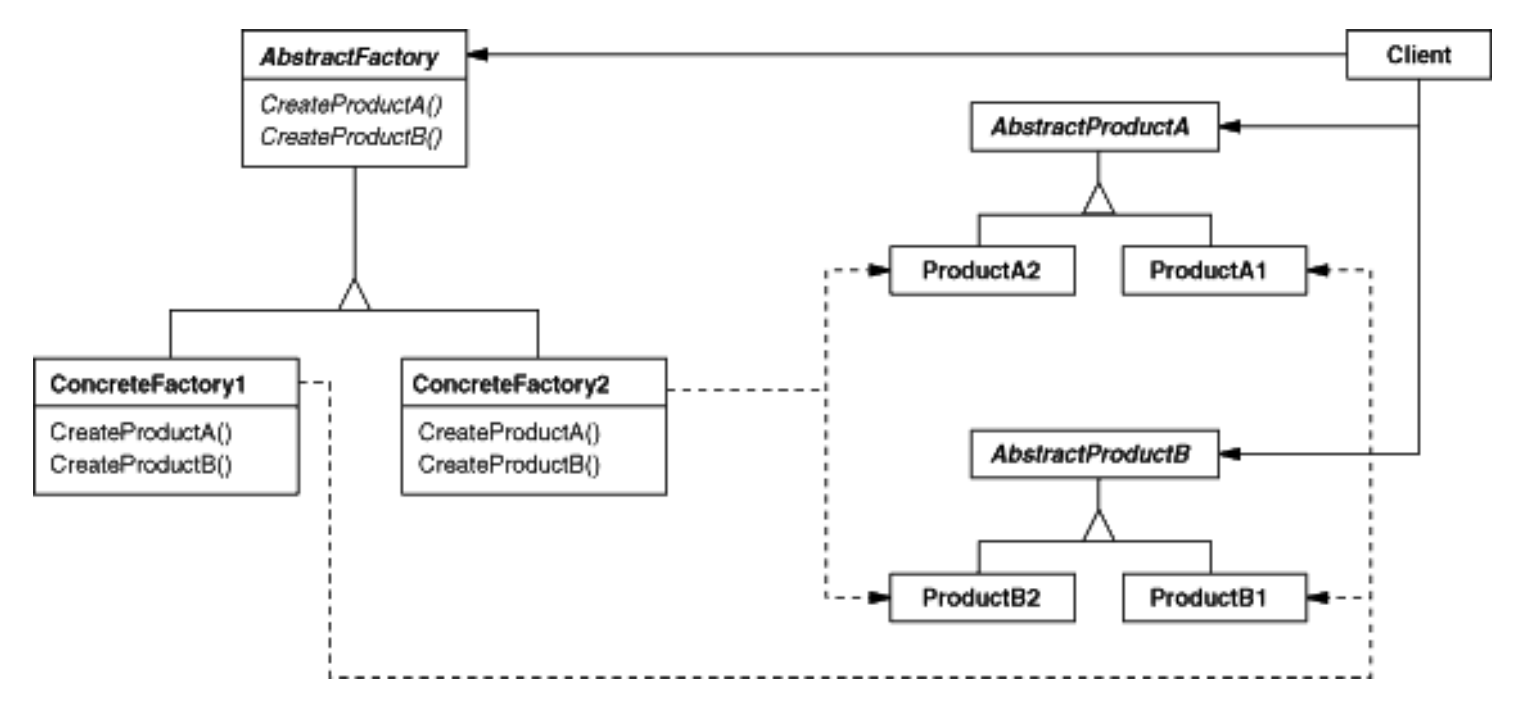
\includegraphics[width=\textwidth]{/Users/matt/Documents/LaTex/Design Pattern LaTex/Command/Structure1}


%---
\section{Timeline}

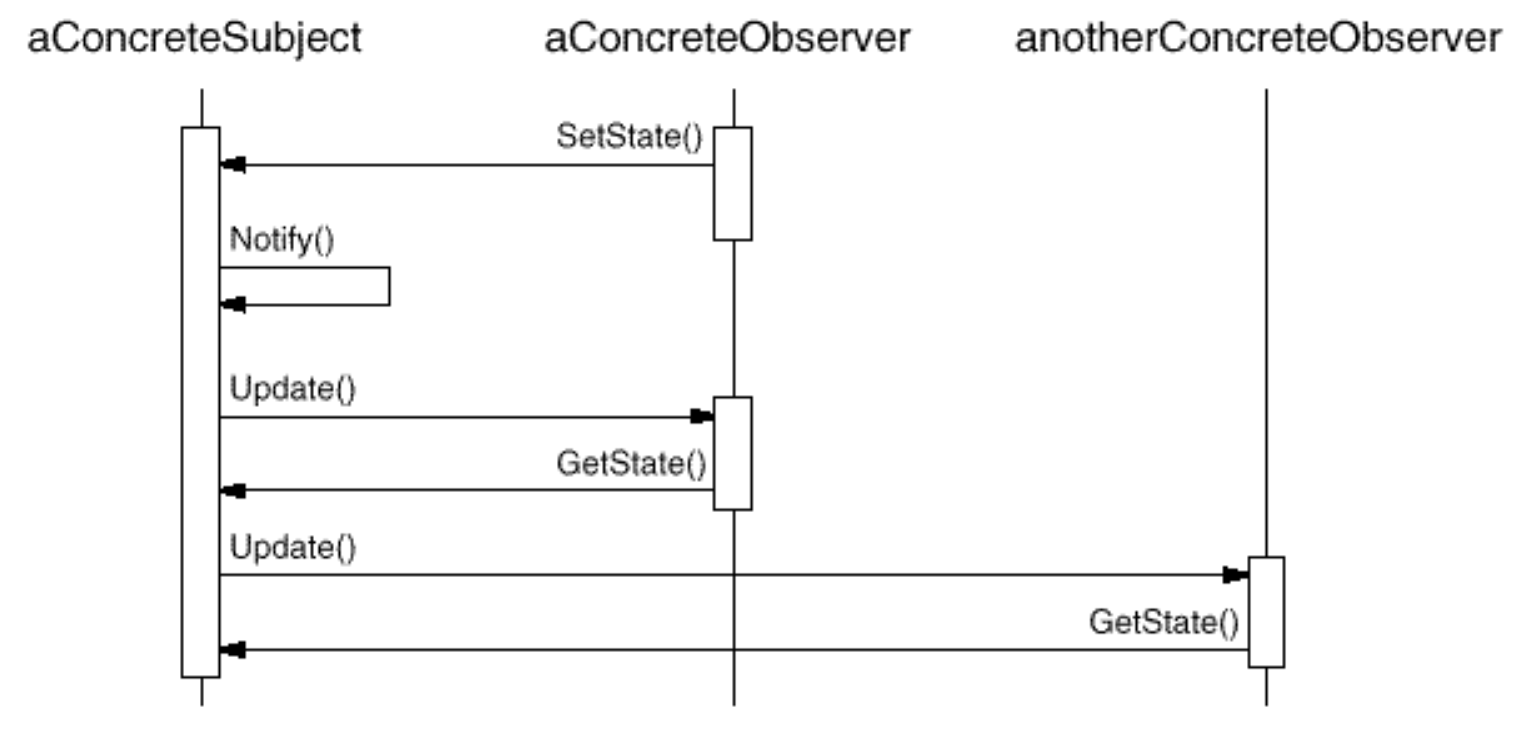
\includegraphics[width=\textwidth]{/Users/matt/Documents/LaTex/Design Pattern LaTex/Command/Timeline1}


%---
\section{Esempio Java}
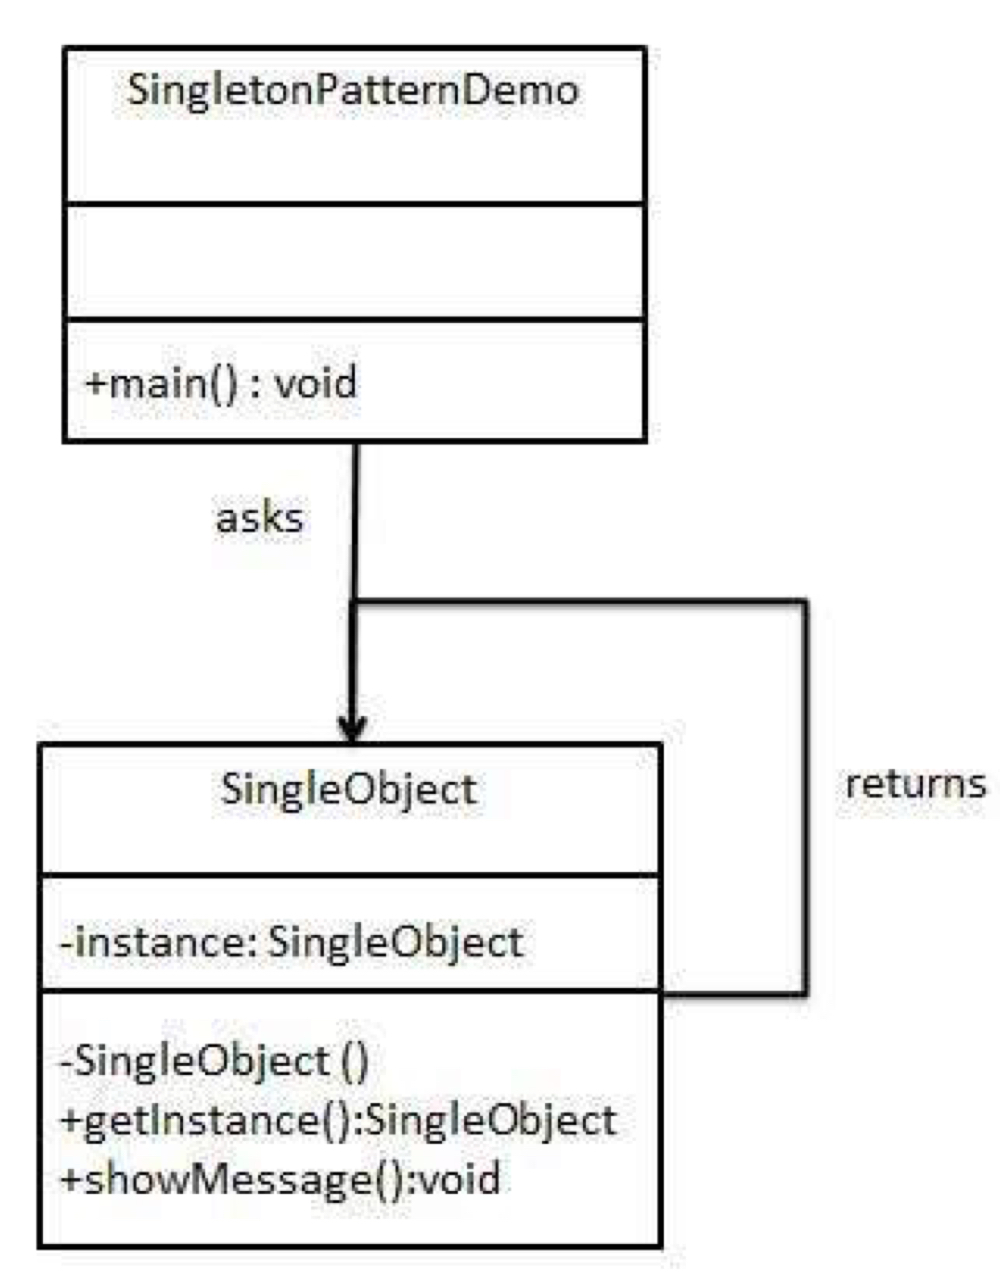
\includegraphics[width=\textwidth]{/Users/matt/Documents/LaTex/Design Pattern LaTex/Command/Example1}

\subsection{Order.java}
\begin{lstlisting}[language=java]
    public interface Order {
        void execute();
    }
\end{lstlisting}

\subsection{BuyStock.java}
\begin{lstlisting}[language=java]
    public class BuyStock implements Order{
        private Stock stock;
    
        public BuyStock(Stock stock) {
            this.stock = stock;
        }
    
        @Override
        public void execute() {
            stock.buy();
        }
        
    }
\end{lstlisting}

\subsection{SellStock.java}
\begin{lstlisting}[language=java]
    public class SellStock implements Order{
        private Stock stock;
    
        public SellStock(Stock stock) {
            this.stock = stock;
        }
    
        @Override
        public void execute() {
            stock.sell();
        }
        
    }
\end{lstlisting}

\subsection{Stock.java}
\begin{lstlisting}[language=java]
    public class Stock {
        private String name;
        private int quantity;
    
        public Stock(String name, int quantity) {
            this.name = name;
            this.quantity = quantity;
        }
    
        public void buy(){
            System.out.println("comprati " + name + " da " + quantity);
        }
    
        public void sell(){
            System.out.println("venduti " + name + " da " + quantity);
        }
    }
\end{lstlisting}

\subsection{Broker.java}
\begin{lstlisting}[language=java]
    public class Broker {
        private List<Order> orderList = new ArrayList<>();
    
        public void takeOrder(Order order) {
            orderList.add(order);
        }
    
        public void placeOrder() {
            for (Order order : orderList) {
                order.execute();
            }
            orderList.clear();
        }
    }
\end{lstlisting}

\subsection{main}
\begin{lstlisting}[language=java]
    public static void main(String[] args) {
        Stock stock = new Stock("prodotti", 10);
    
        BuyStock buyStock  = new BuyStock(stock);
        SellStock sellStock = new SellStock(stock);
    
        Broker broker = new Broker();
        broker.takeOrder(buyStock);
        broker.takeOrder(sellStock);
    
        broker.placeOrder();
    }
\end{lstlisting}